\status{started}
\chapter{muEDM}
\label{ch:muEDM}
\begin{refsection}

{\itshape
This chapter is an introduction to the muEDM experiment. After describing in some detail the spin dynamics, a reminder on the EDM searches for the different particles will follow.
We will then outline the measuring principle of the experiment, the frozen spin technique, and deep dive into the current status of the experiment. 
The study of systematic uncertainties will close this chapter. 
As always, the early stage of the experiment means the rate of changes and improvement is outstanding. 
This my attempt to an up-to-date description but some details might be already outdated.}

\status{review}
\section{Electric Dipole Moment}
    As introduced in \ref{intro:edm}, the Hamiltonian describing the spin dynamics is:
    \begin{equation*}
        \hat{H} = -\mu\bm{\hat{\sigma}\cdot B}-d\bm{\hat{\sigma}\cdot E}
    \end{equation*}
    We then saw that, when considering a combination of magnetic and electric fields and a moving particle it is useful to introduce the polarization vector $\bm{\Pi}=\bm{s}/s$ and the Thomas precession $\bm{\Omega}_0$:
    \begin{equation*}
        \dv{\bm{\Pi}}{t}=\bm{\Omega}_0 \times \bm{\Pi}, \quad
        \bm{\Omega}_0 = -\frac{e}{m\gamma} \left[ (1+\gamma a)\bm{B}-\frac{a\gamma^2}{\gamma+1}(\bm{\beta}\cdot\bm{B})\bm{\beta}-\gamma \left( a+\frac{1}{\gamma+1} \right) \frac{\bm{\beta}\times \bm{E}}{c} \right]
    \end{equation*}
    With no electrical field parallel to the momentum and with $\bm{\Omega}_c$ the cyclotron frequency, the relative spin precession of a muon in a storage ring is described by (T-BMT \cite{miss-59}):
    \begin{equation}
        \begin{split}
            \bm{\Omega}=\bm{\Omega}_0-\bm{\Omega}_c &=
            \underbrace{ 
                \frac{q}{m}\left[ a\bm{B} -{\frac{a\gamma}{\gamma+1}(\bm{\beta}\cdot \bm{B})\bm{\beta}} - \left(  a+\frac{1}{1-\gamma^2}\right)\frac{\bm{\beta} \times \bm{E}}{c} \right]
            }_{\text{Anomalous precession, } \omega_a=\omega_L-\omega_c} \\&+
            \underbrace{
                \frac{\eta q}{2m}\left[ \bm{\beta} \times \bm{B} + \frac{\bm{E}}{c}- {\frac{\gamma c}{\gamma+1}(\bm{\beta}\cdot\bm{E\beta})} \right]
            }_{\text{Interaction of EDM and relativistic $\bm{E}$, } \omega_a}
        \end{split}
        \label{eq:muedm:precession}
    \end{equation}
    The second term describes the precession due to the \gls{edm} coupling to the relativistic $\bm{E}$, perpendicular to the $\bm{B}$ in which the particle is moving. 
    In the presence of a muon \gls{edm} the plane would be tilted and a vertical precession ($\bm{\omega}_e\perp\bm{B}$), shifted by $\pi/2$ to the horizontal anomalous precession, would become observable.

    \status{review}
    \subsection{Symmetry violation}
        In physics, there are three cardinal discrete symmetries: Charge (C), Parity (P), and Time (T).
        P and T are related to the invariance under spatial and temporal reversal while C is the invariance for particle $\leftrightarrow$ \textit{anti}particle exchange.
        While the magnetic field and the spin are \textit{pseudo}-vectors under P and vectors under T, the electric field behaves in the opposite way.
        The implication of this difference is that EDM and MDM behave differently under C, P, and T:
        \begin{equation}
            MDM : 
            \begin{cases}
                \textbf{P} (-\mu\bm{\hat{\sigma}\cdot B}) = -\mu \bm{P(\hat{\sigma}) \cdot P(B)} = -\mu\bm{(+\hat{\sigma})\cdot (+B)} = -\mu\bm{\hat{\sigma}\cdot B} \\
                \textbf{T} (-\mu\bm{\hat{\sigma}\cdot B}) = -\mu \bm{T(\hat{\sigma}) \cdot T(B)} = -\mu\bm{(-\hat{\sigma})\cdot (-B)} = -\mu\bm{\hat{\sigma}\cdot B} 
            \end{cases}
        \end{equation}
        \begin{equation}
            EDM : 
            \begin{cases}
                \textbf{P} (-d\bm{\hat{\sigma}\cdot E}) = -d \bm{P(\hat{\sigma}) \cdot P(E)} = -d\bm{(+\hat{\sigma})\cdot (-E)} = +d\bm{\hat{\sigma}\cdot E} \\
                \textbf{T} (-d\bm{\hat{\sigma}\cdot E}) = -d \bm{T(\hat{\sigma}) \cdot T(E)} = -d\bm{(-\hat{\sigma})\cdot (+E)} = +d\bm{\hat{\sigma}\cdot E}          
            \end{cases}
        \end{equation}
        In light of the CPT theorem, the breaking of the T symmetry implies the breaking of CP.
        
    \status{review}
    \subsection{Current limits on EDM}
        As discussed in \ref{sec:exp:edm}, the last decades saw a continuous effort to measure the EDM of different particles.
        There the experiments setting the current limits were discussed but we report in Tab.~\ref{tab:edm} the results to aid the reader.
        It is important to note there are two limits for $\upmu$: one obtained by rescaling the limit on $d_e$, obtaining an \textit{indirect limit}; one, less stringent, is a \textit{direct} limit ($^*$).

        \begin{table}[h]
            \centering
            \begin{tabular}{|c|c|c|}
                \hline
                Experiment & Particle & EDM limit in ecm \\
                \hline
                \hline
                nEDM \cite{nEDM} & n & \num{0.18e-25}\\
                \hline
                ACME \cite{eEDM:ACME} & e & \num{1.1e-29} \\
                \hline
                Indirect \cite{muEDM:indirect} & $\upmu$ & \num{0.19e-19} $^*$ \\
                \hline
                g-2 \cite{muEDM:direct} & $\upmu$ & \num{1.8e-19} \\
                \hline
            \end{tabular}
            \caption{Sumary of the current limits on the EDM for neutron electron and muon.}
            \label{tab:edm}
        \end{table}

    \status{review}
    \subsection{The \textit{frozen spin} technique}
        
        As illustrated in \cite{1,9}, with the appropriate choice of electric field and having $\bm{p}$, $\bm{B}$ and $\bm{E}$ forming an orthogonal basis, the anomalous precession term in eq. \ref{eq:muedm:precession} can be set to zero. 
        \begin{equation}
            a\bm{B}=\left( a-\frac{1}{\gamma^2-1} \right)\frac{\bm{\beta}\times\bm{E}}{c}
        \end{equation}
        In this situation the relative angle between $\bm{p}$ and spin remains unchanged if $\eta=0$, hence 'frozen'. 
        In the presence of an \gls{edm} the change in polarization would then follow
        \begin{equation}
            \label{eq:freezed}
            \dv{\bm{\Pi}}{t}=\bm{\omega}_e \times \bm{\Pi}, \quad
            \bm{\omega}_e=\frac{\eta q}{2m} \left(\bm{\beta}\times\bm{B}+\frac{\bm{E}_f}{c} \right) =
            \frac{2 d_\mu}{\hbar} \left(\bm{\beta}c\times\bm{B}+\bm{E}_f\right)
        \end{equation}
        The net result of the \gls{edm} is then a vertical build-up of the polarization given by Eq.~\ref{eq:edm:polarization} and illustrated by the sketch in Fig.~\ref{fig:muEDM:g-2_EDM}.
        \begin{equation}
            |\bm{\Pi}(t)|=P(t)=P_0\sin(\omega_e t)\approx P_0 \omega_e t \approx 2P_0\frac{d_\mu}{\hbar}\frac{E_f}{a\gamma^2}t
            \label{eq:edm:polarization}
        \end{equation}    
        At this point, we would like to evaluate the sensitivity to this vertical build-up and this is dependent on the experimental setup investigated.
        \begin{equation}
            \dv{P}{d_\mu}=\frac{2P_0E_ft}{a\hbar\gamma^2}
        \end{equation}     
        \begin{equation}
           \sigma(d_\mu)=\frac{a\hbar\gamma}{2P_0E_f\sqrt{N}\tau_\mu A}
        \end{equation}  
        
       

        \begin{figure}
            \centering
            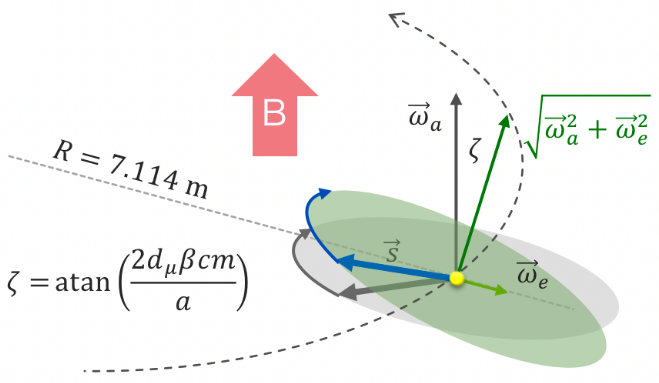
\includegraphics[width = 0.6\textwidth]{Figures/muEDM/g-2_EDM.png}
            \caption{}
            \label{fig:muEDM:g-2_EDM}
        \end{figure}
        
\section{The muEDM experiment}

\status{started}
\section{The precursor}
    The task at hand is quite complex and for this reason, the aim is to first have a working prototype to demonstrate the measuring principles, the achieved control on the different sources of uncertainties and the correct working of the different subdetectors.
    
    \status{started}
    \subsection{Superconducting injection channel}
        To allow the incoming muons to enter the magnet without being reflected or deviated by fringing fields an injection channel is needed.
        For reasons that will be discussed in the section dedicated to the systematics (see Sec.~\ref{muEDM:systematics}), we will actually require two symmetrical injections.
        The idea is to use a superconducting pipe: the fields around the pipe will generate Eddy currents which will, in turn, generate an opposite field inside the pipe, canceling the first.
        Clearly, the development of such a system is not trivial, and a precise study of the different shapes and materials is required. 
        The hope would be to find a suitable \textit{high-temperature} superconductor.

    \status{review}
    \subsection{Entrance detector} 
        After a muon successfully enters the experiment it would spiral to the other side of the magnet. 
        To store it a magnetic kick is necessary. 
        How to produce this kick is going to be discussed in the next section but in either case, this system needs to be triggered.
        To detect the muon entering the system a thin scintillator can be used.
        This needs to be thick enough to produce sufficient light but thin enough not to deflect the particle from the design orbit.
        With a dedicated \gf simulation\footnote{To be honest this was actually my first \gf project and \textit{few iterations} were needed.}, the amount of light exiting the different sides of the thin scintillator was studied as a function of the muon momentum. 
        The results of the simulations and the dedicated beamtimes to develop this entrance detector will be discussed in Ch.~\ref{ch:muEDM:entrance}, dedicated to this detector.

    \status{started}
    \subsection{Muon tracking}
    \label{sec:muEDM:gridpix:beamtime}
        Although during physics runs it is important to minimize the number of interactions of the muon along the path, it is a cardinal step to prove the muons are following the correct path.
        For this reason, a removable muon-tracking device is under development.
        The idea is to use \tpc + \grid.

        \paragraph{Beamtime}
        A prototype of this detector was developed and tested in 2022, the results have been published and can be found in \cite{muEDM:PSI:GridPix}.
        The setup was quite simple: the beam was centered through the TPC and scintillators were used as an external trigger.
        During this testing, the detector was tested at different pressures and voltages, and with different mixtures of gas.
    \status{started}
    \subsection{Kicker}
        The prerequisite for the \textit{frozen spin} is to first store the muon around the design orbit.
        This is achieved by applying a longitudinal kick, canceling the momentum component parallel to the magnetic field.
        The development of this element is non-trivial because of the stringent requirements on the strength, time scale, and residual effects of the kick.
        We started by looking into different shapes and types of coil as well as developing \ltsp simulations of the generating circuit.
        The current version of the circuit is shown in Fig.~\ref{fig:muEDM:kicker:circuit}.
        
        \begin{figure}
            \centering
            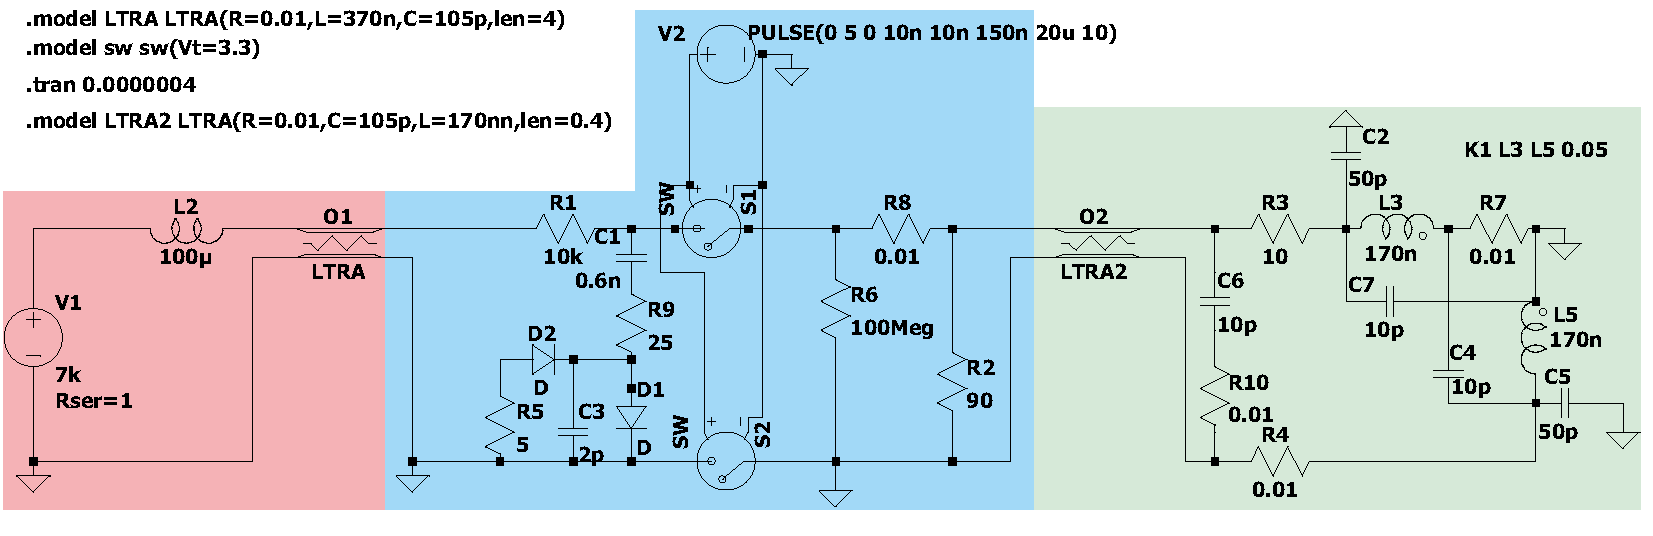
\includegraphics[width = \textwidth]{Figures/muEDM/CircuitMuonKickerV3_1.png}
            \caption{\ltsp simulation for the kicker circuit.}
            \label{fig:muEDM:kicker:circuit}
        \end{figure}

    \status{started}
    \subsection{Electrodes}
        After the muon has been successfully stored around the design orbit the next step is to apply a radial electric field. 
        The strength of this field is going to modify the frequency of the g-2 precession, eventually \textit{freezing} the spin (eq. \ref{eq:freezed}) along the momentum direction.
        These electrodes need to be out of the muon orbit and with a minimal material budget to reduce the positron scattering.  
        Dedicated simulations and prototyping have been developed also for this element.

    \status{review}
    \subsection{Positron tracking}
        The development of the positron tracker has been a big part of my work in the collaboration.
        For this reason, an in-depth description will follow in a dedicated chapter (see Ch.~\ref{ch:muEDM:tracker}) while here we will just outline the basic idea.
        The project is to use two subsystems:
        \begin{outline}
            \1 A silicon pixel external tracker will be used to track precisely the transverse position of the positron. 
            The aim of this sub-detector is to measure the g-2 precession to fine-tune the radial electric field to achieve the frozen-spin condition.
            A straw-tube-based alternative design for this sub-detector is also under study.
            \1 An internal scintillating fiber detector (with comparable resolution on the transverse position) will complement the silicon pixel with additional hits. 
            The requirement is to have a better resolution on the longitudinal position of the hits to measure the EDM by looking at the pitch of the outgoing helical track.
            I dedicated most of my effort to this sub-detector.
        \end{outline}

\section{Systematics}
\label{muEDM:systematics}


\cite{muEDM:Semertzidis:2001} \cite{muEDM:g-2:2008} \cite{muEDM:Adelmann:2010} \cite{muEDM:J-PARC:2011} \cite{muEDM:J-PARC:2016} \cite{muEDM:PSI:2021} \cite{muEDM:PSI:Mikio:2022} \cite{muEDM:PSI:Kim:2022}

\status{review}
\section{Schedule}
    As we just saw, although the development of the precursor is moving at a very nice speed, the tasks are very challenging.
    To put in perspective the current understanding of the different challenges and time constraints, we add here the schedule that was included in the proposal of the experiment in 2022.
    Fig.~\ref{fig:muEDM:schedule:short} is a schedule on the short period up to the long shut-down, in which 6 main milestones are highlighted:
    \begin{outline}
        \1[1] Demonstration of off-axis injection
        \1[2] Muon selection and generation of trigger
        \1[3] Generation of the pulsed magnetic field and measurement of eddy-currents
        \1[4] Stopping of muons and detection of $(g - 2)$ precession
        \1[5] Adjusting the electric field by tuning $(g - 2)$ precession to zero
        \1[6] Data-taking in muon EDM mode
    \end{outline}
    Fig.~\ref{fig:muEDM:schedule:long} goes beyond the long shut-down and covers the full life of the experiment, up to 2033.
    
    \begin{figure}
        \centering
        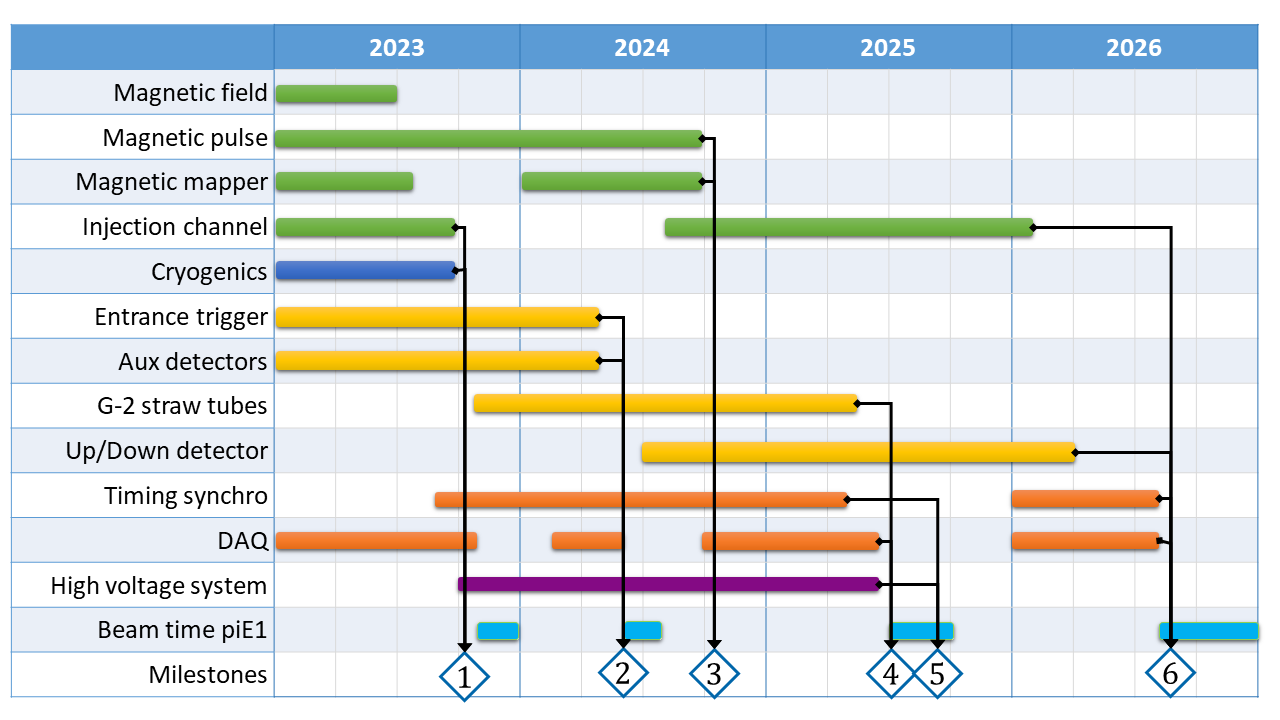
\includegraphics[width = \textwidth]{Figures/muEDM/Schedule2023-2026.png}
        \caption{`Short' term muEDM schedule, with highlighted the 6 main milestones up to the \textit{long shutdown}. Milestones: 1) off-axis injection; 2) generation of the entrance trigger; 3) generation of the pulsed B field; 4) detection of $g-2$; 5) adjust $g-2$ to zero; 6) EDM data taking.}
        \label{fig:muEDM:schedule:short}
    \end{figure}
       
    \begin{figure}
        \centering
        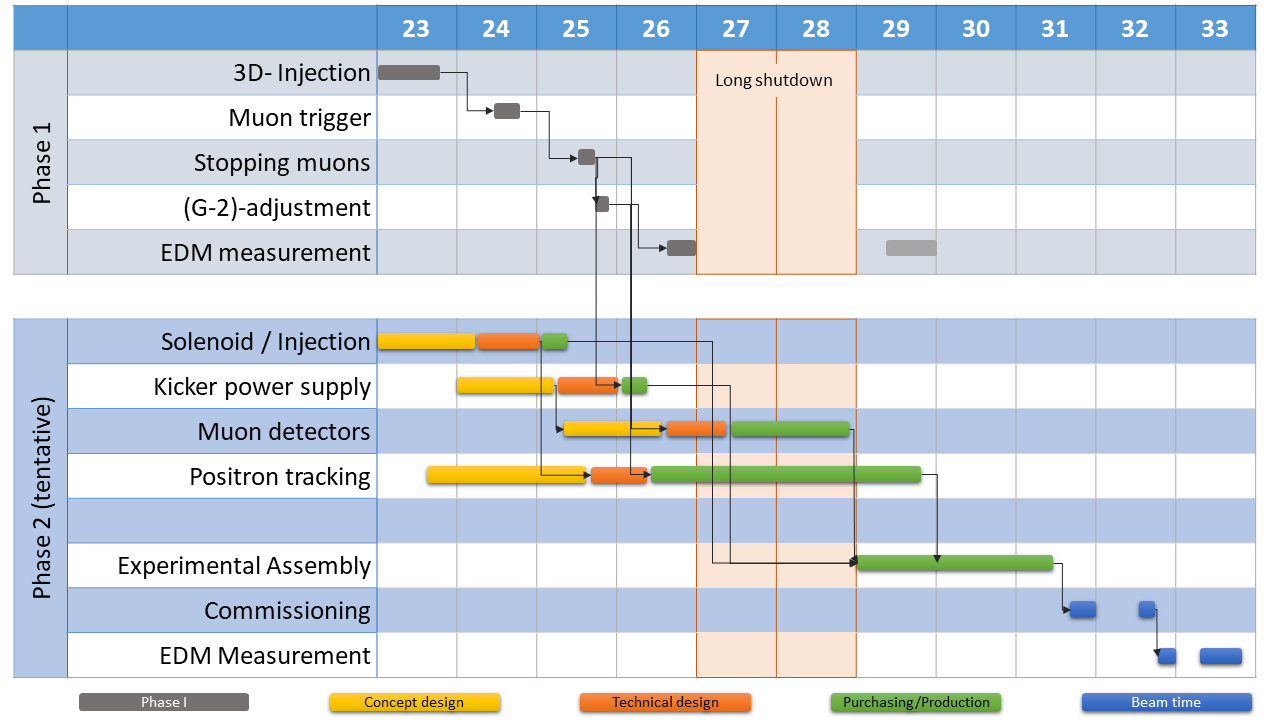
\includegraphics[width = \textwidth]{Figures/muEDM/SchedPropLongTerm23.png}
        \caption{`Long' term muEDM schedule, with the different phases up to the end of the experiment.}
        \label{fig:muEDM:schedule:long}
    \end{figure}
    
\section{Conclusions}

\status{started}
\printbibliography[
    heading = bibliographychapter,
    title=Bibliography on muEDM
]

\end{refsection}
